\section{WebPosTransaction.java Class}
The performed \emph{Code Inspection} activity has been focused on the \emph{WebPosTransaction.java} class. That class is related to the \emph{webpos} package which contains a plugin that may be integrated with other functionalities provided by \textit{OFBiz} in order to provide to the user functionalities related to the management of a web-POS: a browser based Point of Sale solution.

The complete source path of the class in the release 16.11.01 of the \emph{Apache OFBiz project} is:\\

\centerline{\tt apache-ofbiz-16.11.01/specialpurpose/webpos/src/main/java/}
\centerline{\tt /org/apache/ofbiz/webpos/transaction/WebPosTransaction.java} \hfill

The class is located in the package:\\
\centerline{\tt org.apache.ofbiz.webpos.transaction}

\subsection{The \texttt{webpos} package}
This package is related to a plugin that may be integrated with the \emph{Apache OFBiz} suite of applications.\\
It is composed by three main subpackage and a java class:
\begin{itemize}
	\item \texttt{org.apache.ofbiz.webpos.}\textbf{search} package\\Contains a java class to manage some searching functionalities (e.g. about facilities and products).
	\item \texttt{org.apache.ofbiz.webpos.}\textbf{session} package\\Contains a java class representing a web pos session.
	\item \texttt{org.apache.ofbiz.webpos.}\textbf{transaction} package\\Contains a java class representing  a single web pos transaction.
	\item \texttt{org.apache.ofbiz.webpos.}\textbf{WebPosEvents.java} class\\Java class to manage incoming requests from the related web based application.
\end{itemize}

\subsection{Functional Role of the Class}
The \emph{WebPosTransaction.java} class doesn't have any form of documentation or \emph{Javadoc} (\url{https://ci.apache.org/projects/ofbiz/site/javadocs}) making really hard the comprehension of its functionalities from a source code analysis.

For these reasons we will provide a high-level overview of the functionality role of the class in relation with related java classes. The description provided is based upon our interpretation of the source code, some documentation about other classes of the project and UML class diagrams generated from the code, so it may not correspond entirely to a right description of the intention of the java class author.\\

\clearpage

The \emph{WebPosTransaction.java} class identifies a single transaction in the context of a \emph{WebPosSession}. The transaction is also related to a \emph{ShoppingCart} object, held by the session, and its methods allow to manage the payment procedure also instantiating the order related to the cart checkout. \\

In \autoref{fig:package} are shown relations of other components in the \emph{webpos} package with respect to the \emph{WebPosTransaction.java} class:
\begin{itemize}
	\item The \emph{WebPosEvents} class has a method \emph{completeSale} that after obtaining the current transaction through the \emph{getCurrentTransaction} method (exposed by the \emph{WebPosSession}) interacts with it calling the \hyperref[method:processSale]{\emph{processSale}} method
	\item The \emph{WebPosSession} class has a field \emph{webPosTransaction} that stores the current transaction related to the session
	\item The \emph{WebPosSession} class has three methods that interacts with the transaction stored as a field: \emph{getCurrentTransaction}, \emph{setCurrentTransaction} and \emph{logout}
\end{itemize}

\begin{figure}[h]
			\centering
			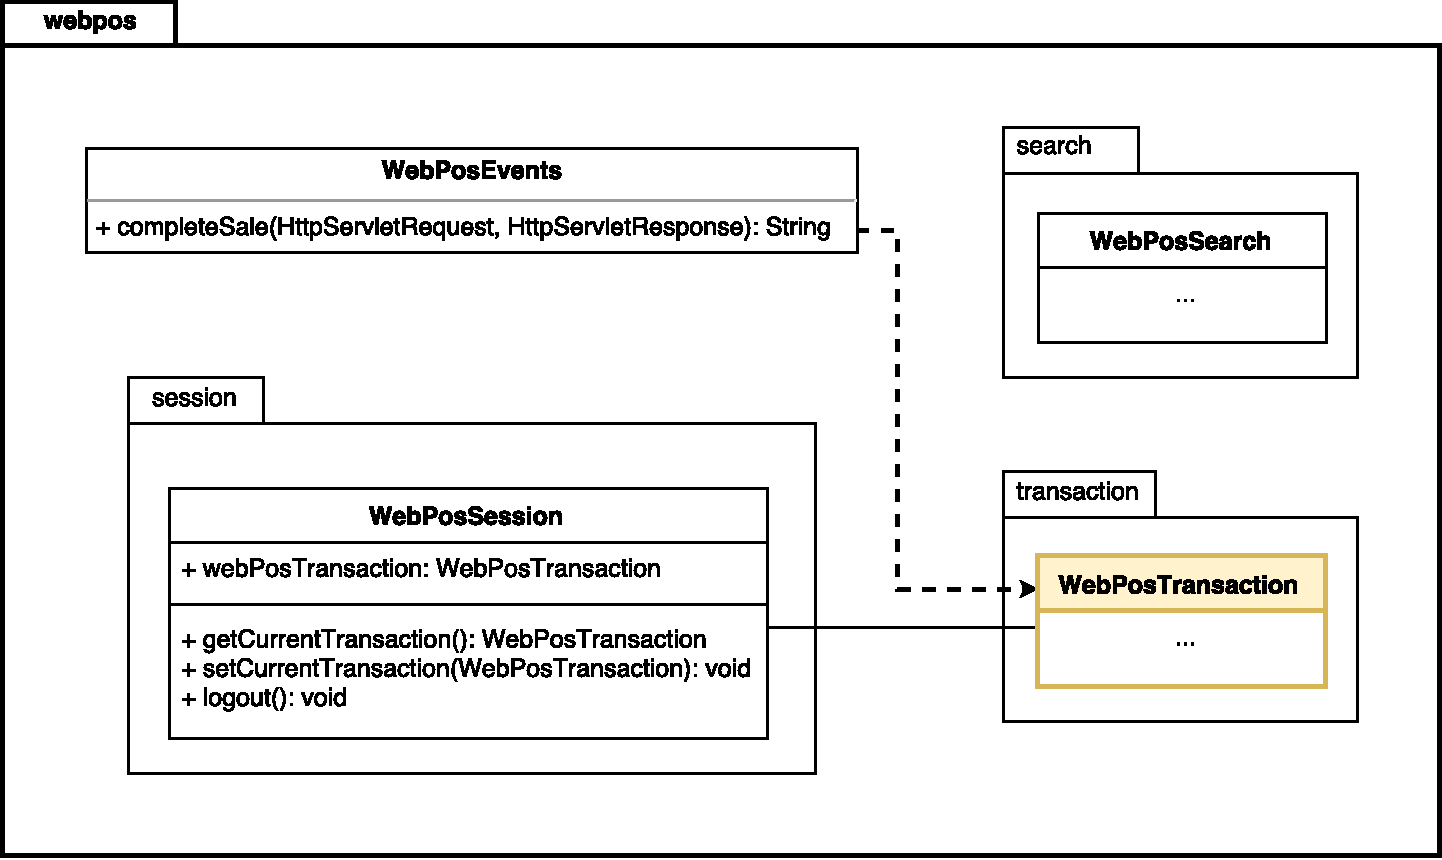
\includegraphics[width=0.8\linewidth]{package}
			\caption{
				\label{fig:package} 
				\emph{WebPosTransaction.java} relations inside the \emph{webpos} package
			}
\end{figure}

The \emph{WebPosTransaction.java} is dependent on the \emph{WebPosSession} related:
\begin{itemize}
	\item A \emph{WebPosTransaction} object needs a \emph{WebPosSession} instance to be instantiated through the constructor
	\item A \emph{WebPosTransaction} instance has as field a related \emph{WebPosSession} instance
	\item Many methods of the \emph{WebPosTransaction} class rely on methods (especially getters) of the \emph{WebPosSession} instance related
\end{itemize}

\clearpage

\subsection{Class Description}
The \emph{WebPosTransaction} class contains the logic to manage a transaction related to a web pos operation, but the specified methods are supposed to be called from an higher level component holding the transaction object.

\paragraph{Notes} Some notes about concepts used inside the \emph{OFBiz} project:
\begin{itemize}
 	\item An Entity is a relational data construct that contains any number of Fields and can be related to other entities \cite{OFBiz}. Entities are managed by the \emph{entity engine} to be used from java classes transparently from their actual implementation.
 	\item \emph{Generic Entity Value Object} Object that handles persistence for any defined entity (javadoc of \texttt{org.apache.ofbiz.entity.GenericValue})
\end{itemize}

\subsubsection{Fields}
The main fields of the class (excluding constant \emph{final static} fields)  are \emph{private} fields:

\begin{itemize}
    \item \textbf{CheckOutHelper ch} instance of \\ \texttt{org.apache.ofbiz.order.shoppingcart.CheckOutHelper}: an object that provides functionalities to manage the cart related to the order in the checkout phase.
    \item \textbf{GenericValue txLog} instance of \\ \texttt{org.apache.ofbiz.entity.GenericValue}: persistent entity identifying a \emph{PosTerminalLog}, a logger where are stored logs about the transaction
    \item \textbf{String transactionId}: a string to store the identifier of the transaction
    \item \textbf{String orderId}: a string to store the identifier of the order related to the transaction
    \item \textbf{String partyId}: a string to store the identifier of the party, always set as not available (\emph{\_NA\_}) in the current  implementation
    \item \textbf{boolean isOpen}: set as \texttt{true} if there exist a \emph{PosTerminalState} opened
    \item \textbf{int drawerIdx}: field not used in the current implementation of the class, the related getter always return 1
    \item \textbf{GenericValue shipAddress} instance of \\ \texttt{org.apache.ofbiz.entity.GenericValue}: persistent entity identifying the \emph{PostalAddress} entity related to the shipping address
    \item \textbf{WebPosSession webPosSession} instance of \\ \texttt{org.apache.ofbiz.entity.GenericValue}: the current session managing the transaction
\end{itemize}
\clearpage
\subsubsection{Methods}

The main methods of the class (excluding getter methods and methods which functionalities are based upon a unique call to a method external to the class) are \emph{public} methods:

\begin{itemize}
	\item \texttt{public} \textbf{WebPosTransaction}\texttt{(WebPosSession session)} constructor \\
	The class constructor:
	\begin{itemize}
	 	\item set as field the \emph{WebPosSession} given as parameter
	 	\item set the partyId field as \emph{\_NA\_}
	 	\item create a new instance of \emph{CheckOutHelper} passing to its constructor the \texttt{org.apache.ofbiz.entity.}\emph{Delegator} and the \\ \texttt{org.apache.ofbiz.order.shoppingcart.}\emph{ShoppingCart} related to the session
	 	\item update \emph{ShoppingCart} instance w.r.t. information about the session: set channel type as POS\_SALES\_CHANNEL, facility ID, terminal ID and, if the session is associated with a \emph{userLogin} entity, associates the party to the order identifying its role as SALES\_REP
	 	\item set up the transaction logger
	 \end{itemize}
	\item \texttt{public boolean} \textbf{isOpen}\texttt{()} \\
This method returns \texttt{true} if the \emph{getTerminalState} method returns a terminal state  with \textit{closedDate} parameter \texttt{null}, that is if the terminal is open.
	\item \texttt{public GenericValue} \textbf{getTerminalState}\texttt{()} \\This method returns the most recent \emph{PosTerminalState} entity associated to the \emph{terminalId} and \emph{transactionId}.
	\item \texttt{public void} \textbf{closeTx}\texttt{()} \\ This method closes the transaction logger and calls the \emph{clear} method on the \textit{ShoppingCart} instance associated to the session.
   \item \texttt{public void} \textbf{paidInOut}\texttt{(String type)} \\ This method logs the pos transaction as paid together with the \emph{type} string given as parameter and the current date. It also sets the current transaction of the section as \texttt{null}.
   \item \texttt{public void} \textbf{modifyPrice}\texttt{(int cartLineIdx, BigDecimal price)} \\ This method modifies the price of the item identified by the \emph{cartLineIdx}, given as parameter, in the \emph{ShoppingCart} related to the session. The new price for the item is the \emph{price} given as parameter.
   \item \label{method:processSale} \texttt{public BigDecimal} \textbf{processSale}\texttt{() throws GeneralException}\\
   This method is the most complex of the class and involves many external object (as shown in \autoref{fig:processSale}), main purpose of the method can be sketched as:
   \begin{itemize}
   		\item attach the party ID to the cart
    	\item validate payment methods (if it fails throws a \texttt{GeneralException})
    	\item store the order (if it fails throws a \texttt{GeneralException})
    	\item process the payment(s) (if it fails throws a \texttt{GeneralException})
   		\item save the TX Log
   		\item get the change due and return it
   \end{itemize}
   \textbf{Note} This method contains \emph{todo} comments related to functionalities not already implemented
   \item \texttt{private synchronized GenericValue} \textbf{getStoreOrgAddress}\texttt{()} \\ This \emph{synchronized} method returns the \emph{PostalAddress} entity of the facility location related to the session (to be used for tax calculation).
   \item \texttt{public int} \textbf{checkPaymentMethodType}\texttt{(String paymentMethodTypeId)} \\ This method returns the int code related to the type of payment method (NO\_PAYMENT, INTERNAL\_PAYMENT, EXTERNAL\_PAYMENT) based upon the paymentMethodTypeId given as parameter.
   \item \texttt{public String} \textbf{makeCreditCardVo}\texttt{(String cardNumber, String expDate, String firstName, String lastName)} \\ This method creates a \textit{generic entity \textbf{v}alue \textbf{o}bject} related to the credit card described through parameters given as input to the method and returns the \textit{paymentMethodId} related
\end{itemize}

The \autoref{fig:processSale} shows method calls made by the \emph{ProcessSale} method: calls on \textit{java.util} classes have been omitted, calls on both static and not static methods are reported as well as other methods called on the \emph{WebPosTransaction} class.

\begin{figure}[h]
			\centering
			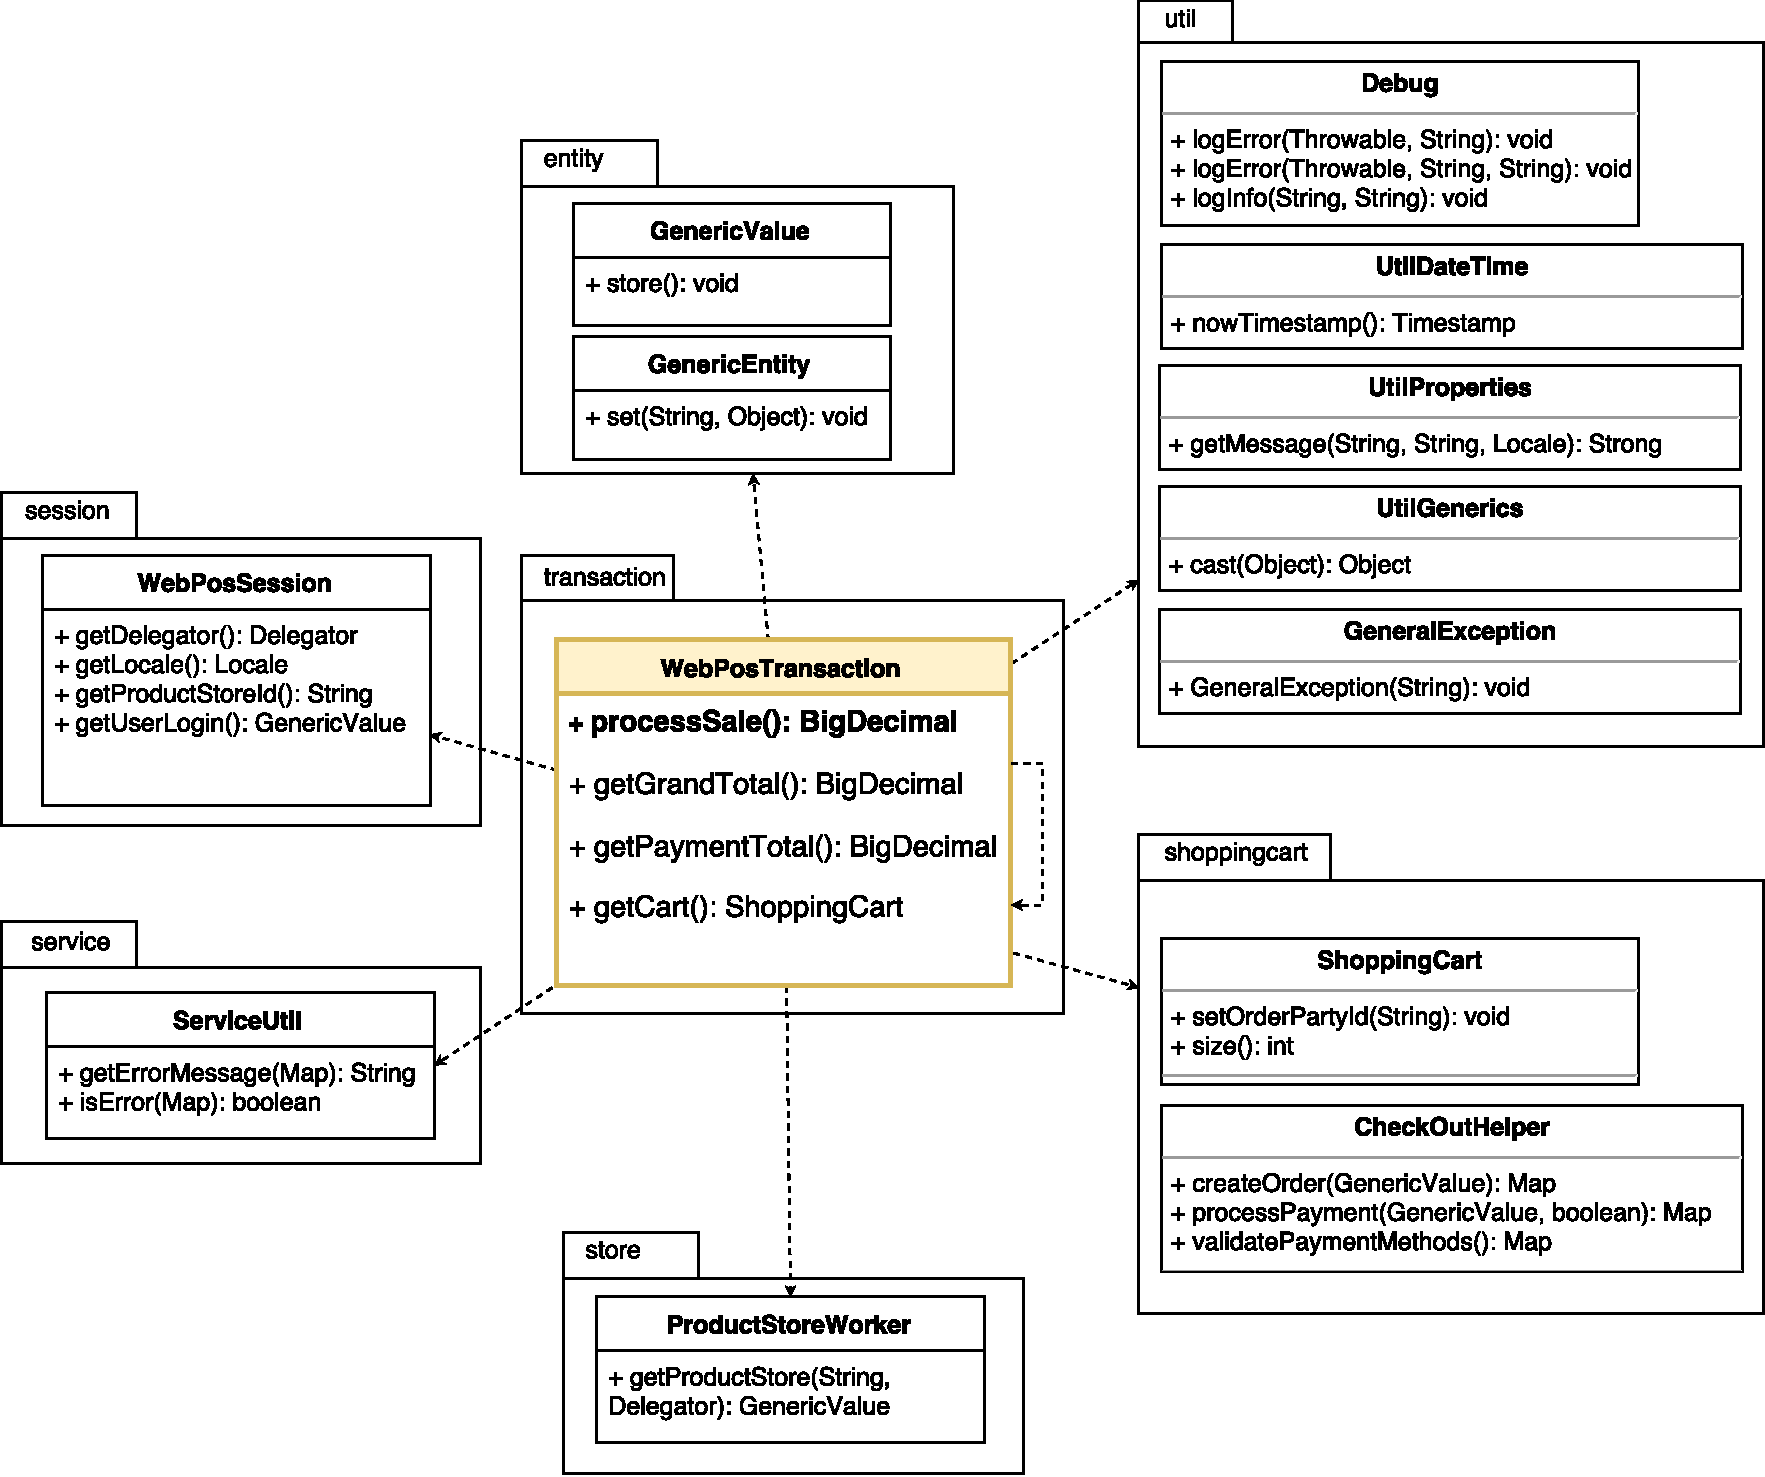
\includegraphics[width=0.85\linewidth]{processSale}
			\caption{
				\label{fig:processSale} 
				\emph{ProcessSale} method
			}
\end{figure}